\documentclass{article}
\usepackage{mystyle}

\title{Notes on HARDI data preprocessing: Effect on tensor fit}
\author{Scott Trinkle}
\date{Last edited: \today}

\begin{document}
\maketitle

These notes describe the effect of data denoising on the resulting tensor
fit, using the principal diffusion direction (PDD) and fractional anisotropy (FA)
as comparison metrics.

Tensor fitting was performed using the FSL
\href{https://fsl.fmrib.ox.ac.uk/fsl/fslwiki/FDT/UserGuide}{dtifit} tool on the
raw data, as well as on the data denoised with sliding windows of
$5\times 5\times 5$, $7\times 7\times 7$, and $9\times 9\times 9$. For this
comparison, the volumes were not registered before computing the tensor fit.

Figure~\ref{fig:FA} shows histograms of the percent difference in FA between the
raw and denoised volumes for each window size, calculated as
\begin{align}
  \Delta \text{FA} = \frac{\text{FA}_{\text{denoised}} - \text{FA}_{\text{raw}}}{\text{FA}_{\text{raw}}} \times 100.
\end{align}
A binary mask was created for the brain using the FSL
\href{https://fsl.fmrib.ox.ac.uk/fsl/fslwiki/BET/UserGuide}{BET} tool on the
averaged $\bar{b}_0$ volume from the $7\times 7\times 7$ denoised volume. All
comparisons were restricted to this mask.

\begin{figure}[h]
  \centering
  \captionsetup{width=0.6\linewidth}  
  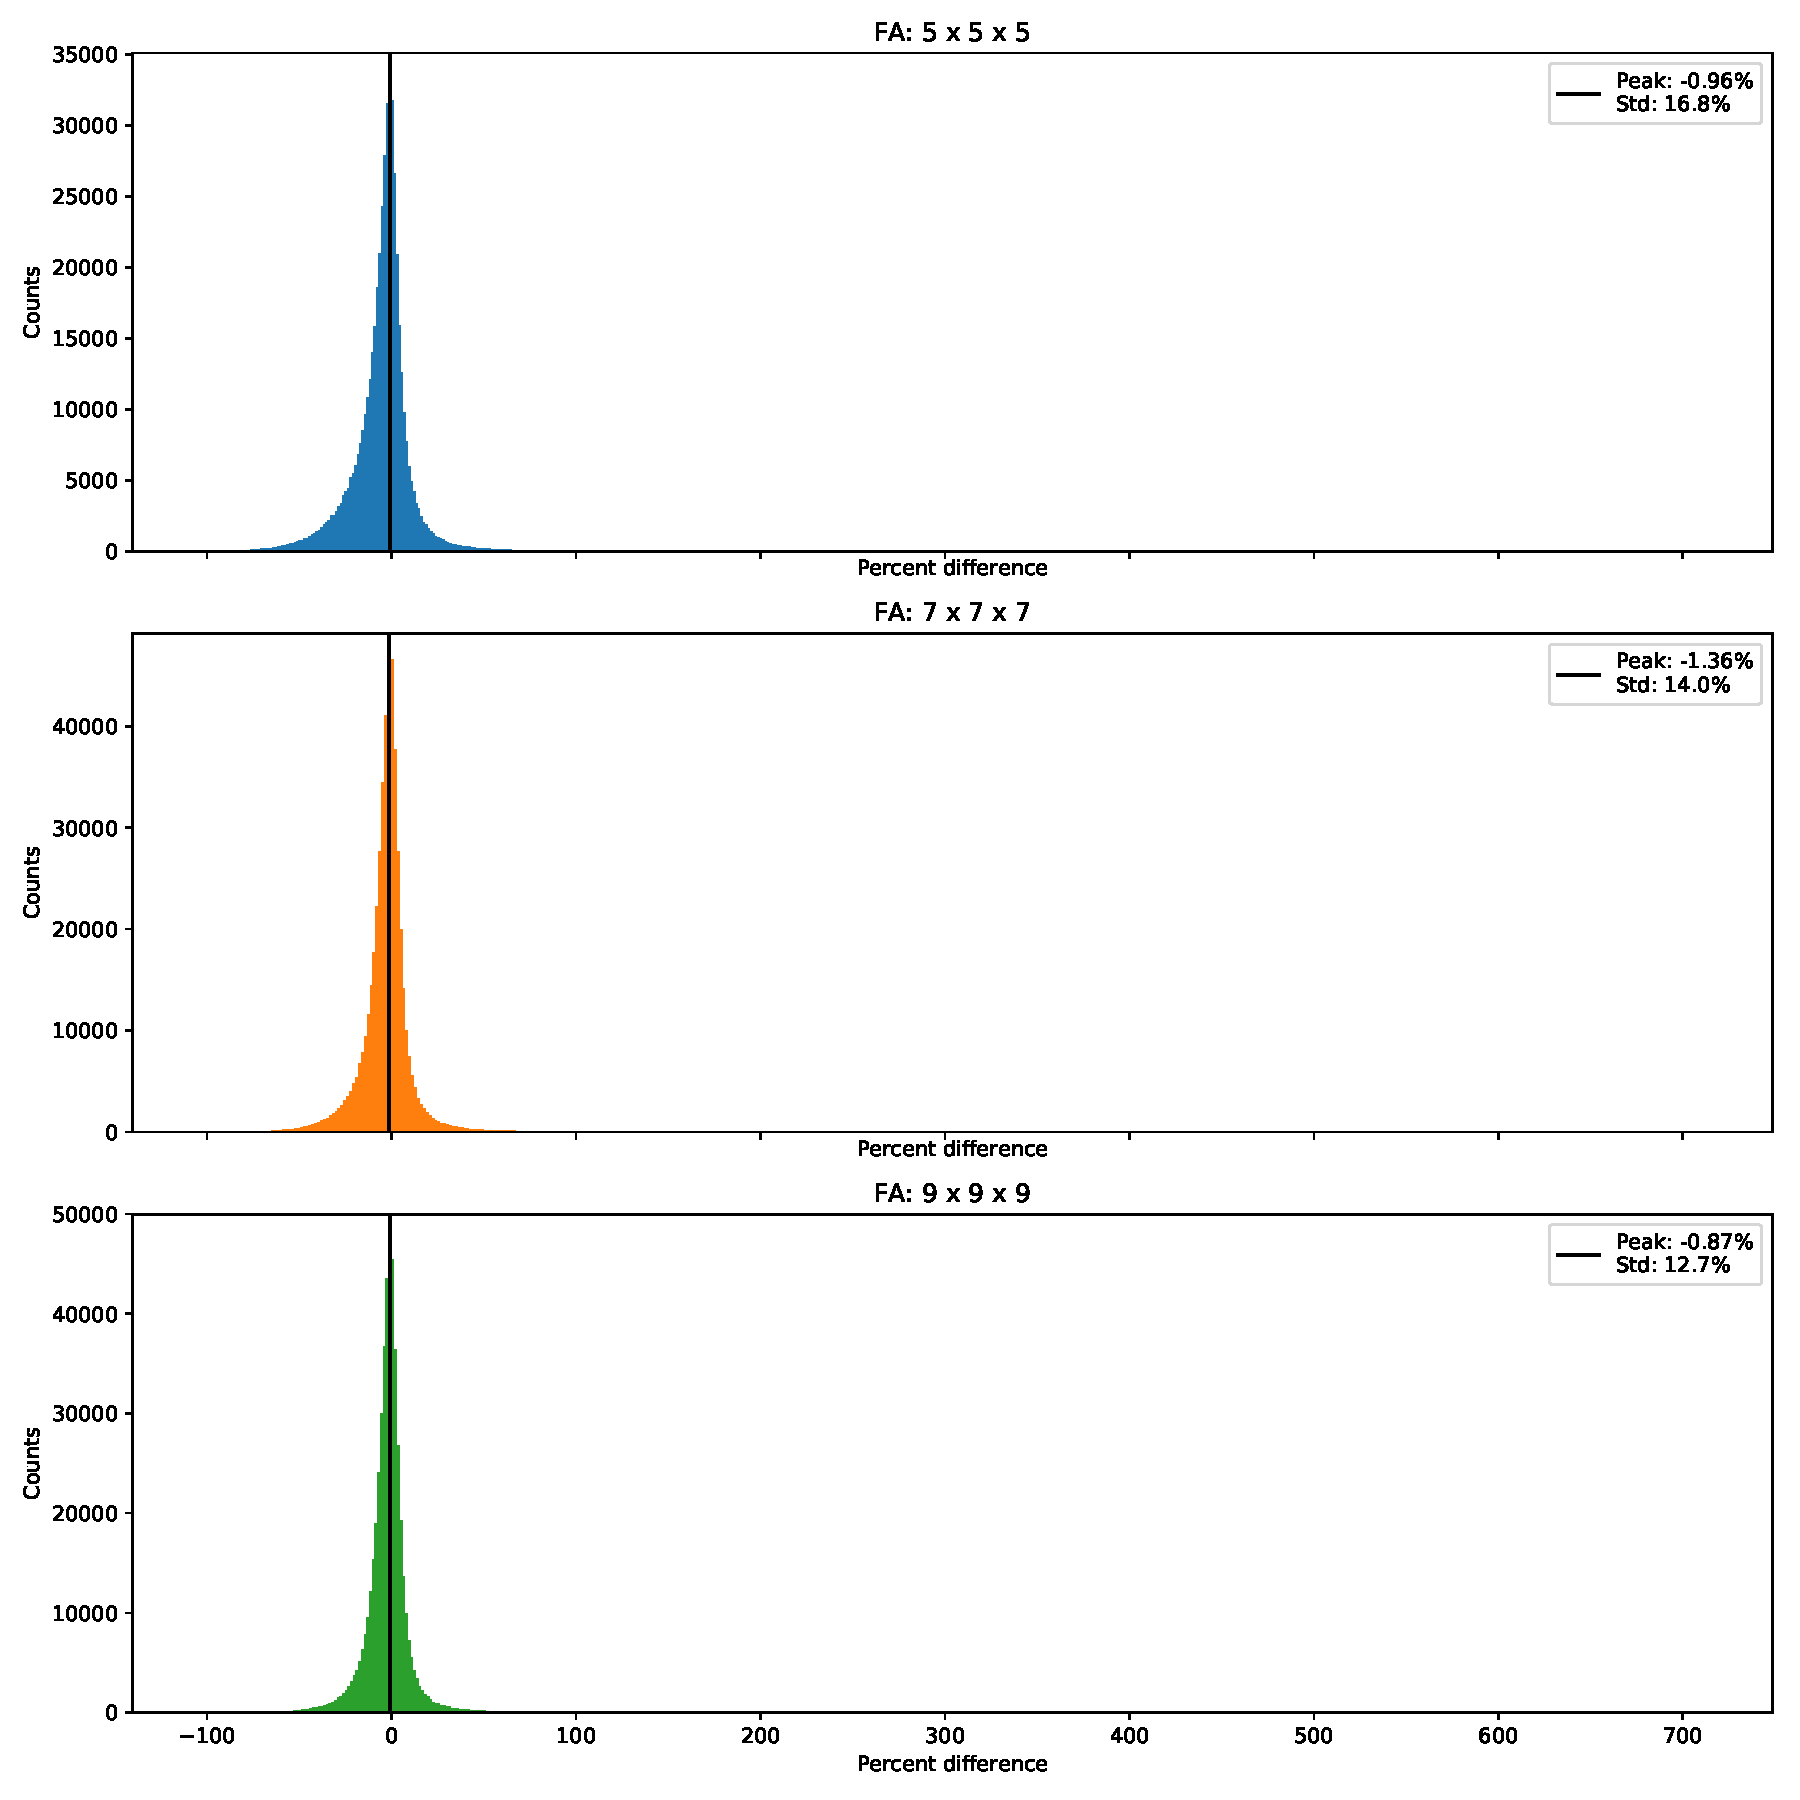
\includegraphics[width=0.6\linewidth]{../figs/noreg_fa}
  \caption{Difference in FA between raw tensor fit and the denoised tensor fits
    with different window sizes. The bold line indicates the peak of the
    distribution. Comparisons were restricted to voxels within the brain. }
  \label{fig:FA}
\end{figure}

Overall, FA differences for all of the denoised volumes were around 1\%. The
anomolous counts (up to 600-700\%) resulted from background voxels being included
in the brain mask. Generally, the distributions get wider with smaller window
sizes.


\begin{figure}[h]
  \centering
  \captionsetup{width=0.6\linewidth}
  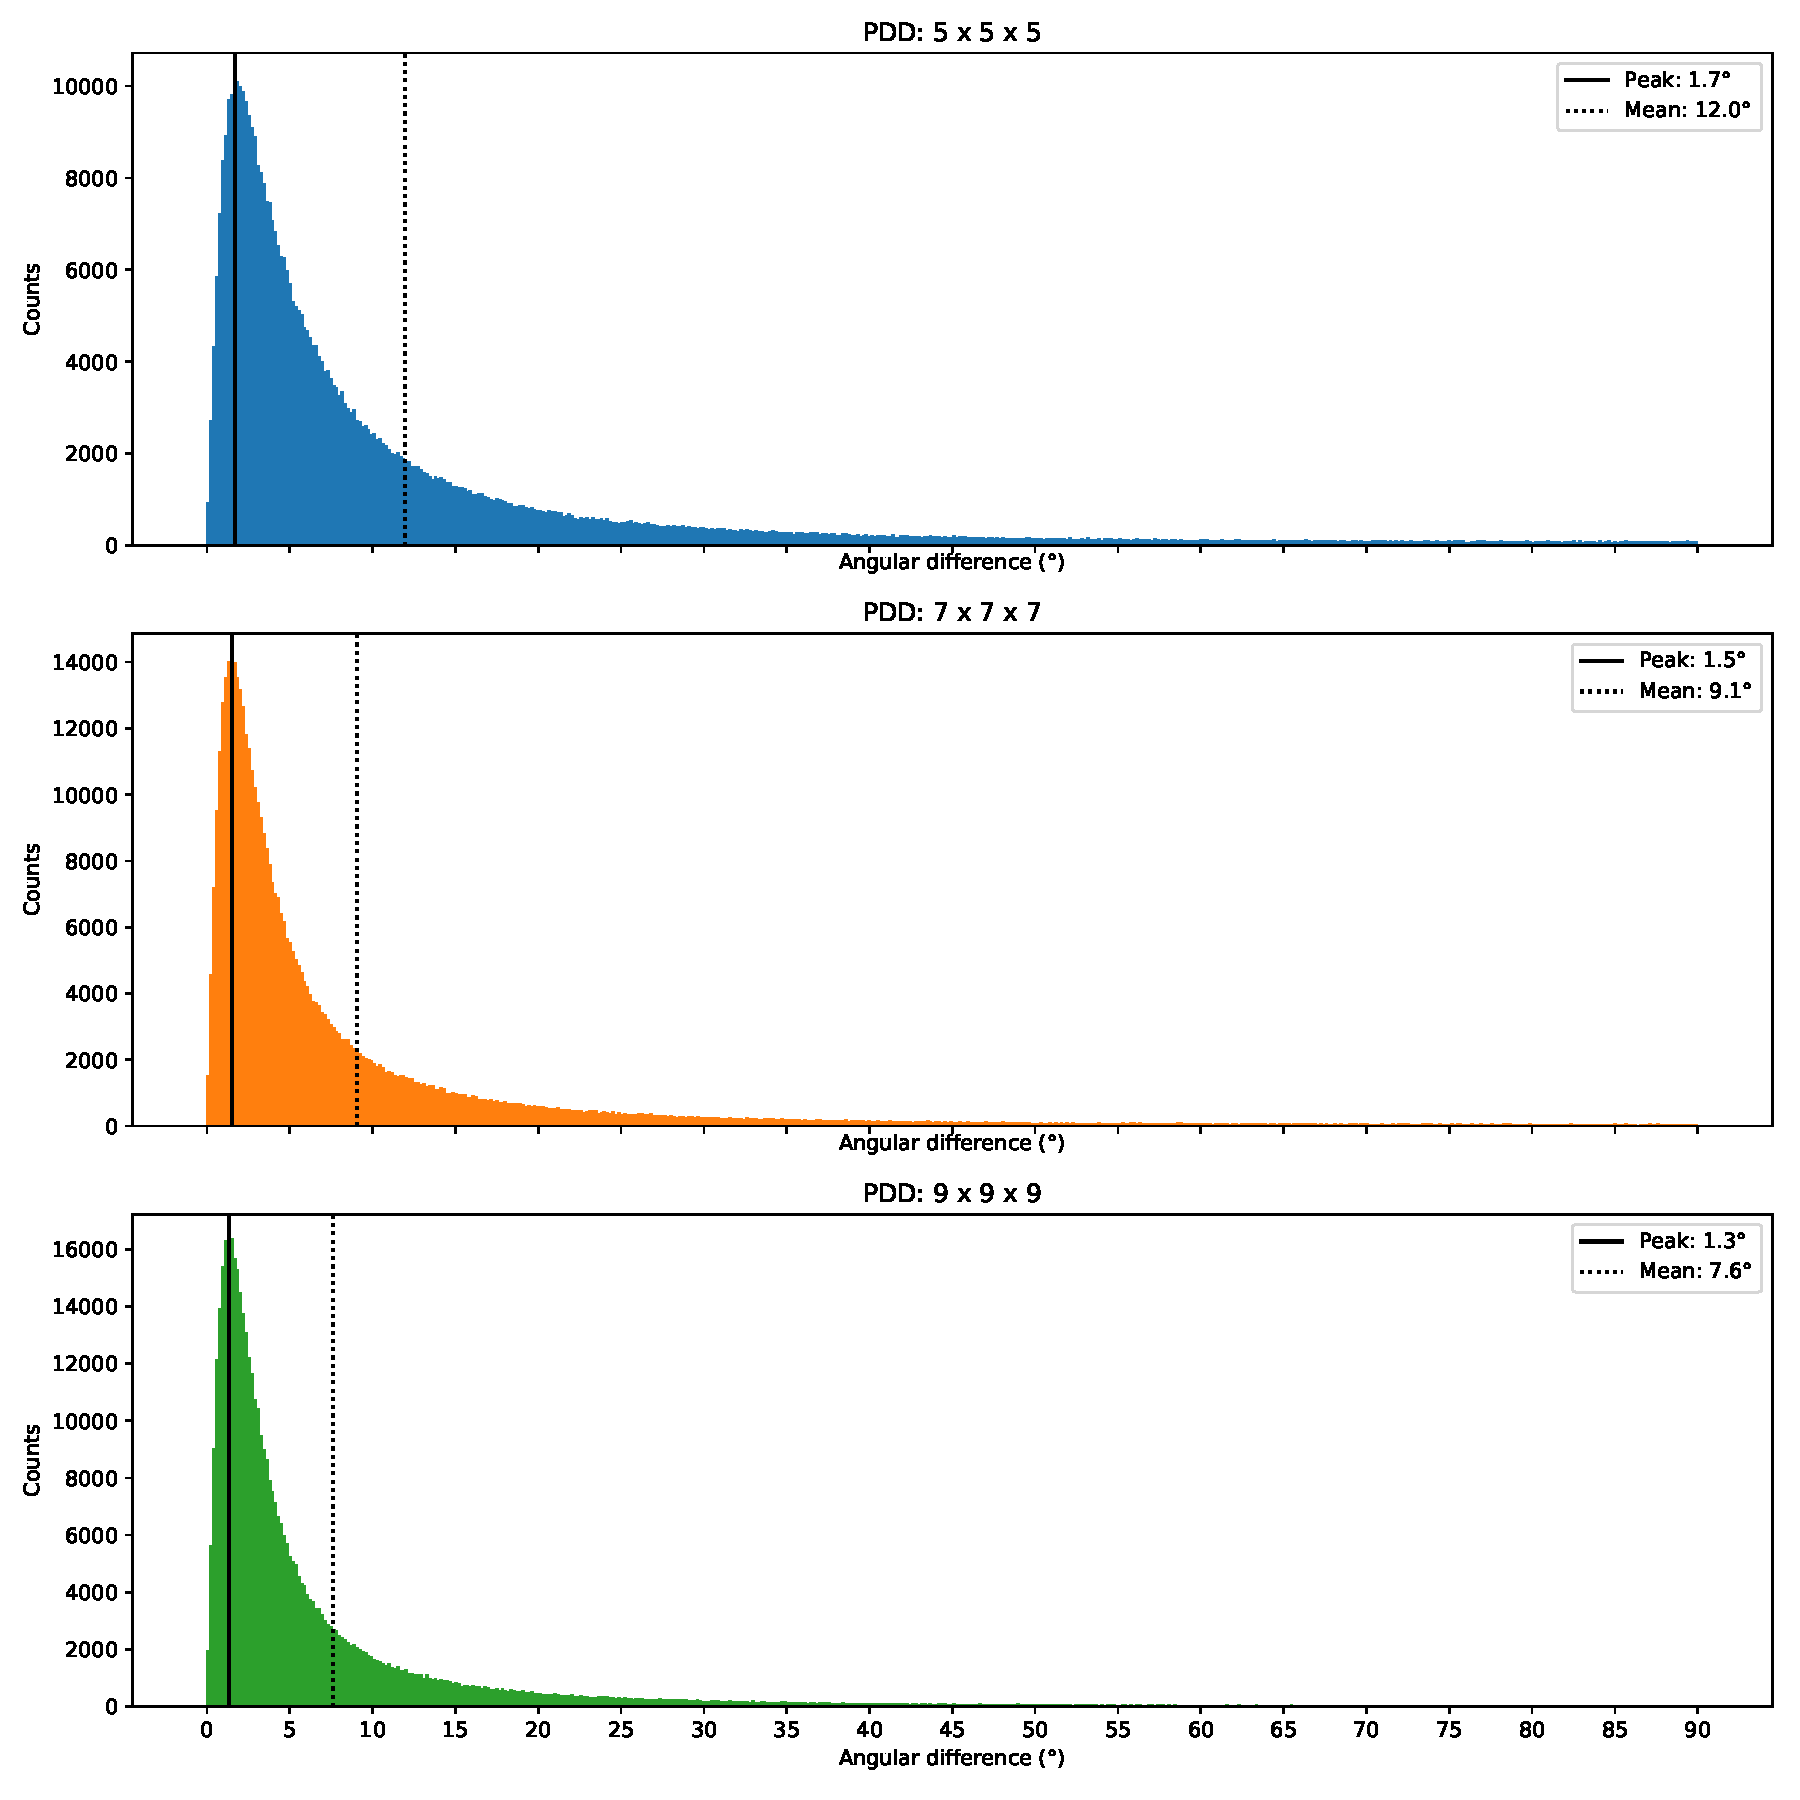
\includegraphics[width=0.6\linewidth]{../figs/noreg_pdd}
  \caption{Angular difference in PDD between raw tensor fit and the denoised
    tensor fits with different window sizes. The bold line indicates the mean
    of the distribution, while the dotted line indicates the mean. The
    Comparisons were restricted to voxels within the brain.  Note that the PDD
    at each voxel is unique within a minus sign, so angular differences are
    restricted to [0$^{\circ}$, 90$^{\circ}$].}
  \label{fig:pdd}
\end{figure}


Figure~\ref{fig:pdd} shows histograms of the angular difference in PDD between
the raw and denoised volumes for each window size. Note that the PDDs are
unique within a minus sign, so the angular differences are restricted to
[0$^{\circ}$, 90$^{\circ}$]. The distributions have similar peaks of about
1.5$^{\circ}$ for each window size, with means increasing from
7.6$^{\circ}$---12.0$^{\circ}$ as the window sizes
decrease. Figure~\ref{fig:pdd_famask} restricts the PDD comparisons to voxels
with FA$>$0.7. Here, we see similar trends with a much lower spread in the
distributions, indicating that denoising has less of an effect on PDD for high
FA voxels (presumably white matter).

Figure~\ref{fig:screenshot} shows spatial maps of PDD angular difference, $b_0$
intensity, and FA difference (from left to right, respectively). These images
confirm the potential trend from comparisons of Figures~\ref{fig:pdd}
and~\ref{fig:pdd_famask}: regions with low angular differences correspond to
regions of high FA and vice versa. In other words: the highest angular
differences generally occur in either gray matter or in the ventricles (where
diffusion is more isotropic), while the lowest differences occur in the white
matter, with more oriented structure.

\begin{figure}[h]
  \centering
  \captionsetup{width=0.6\linewidth}
  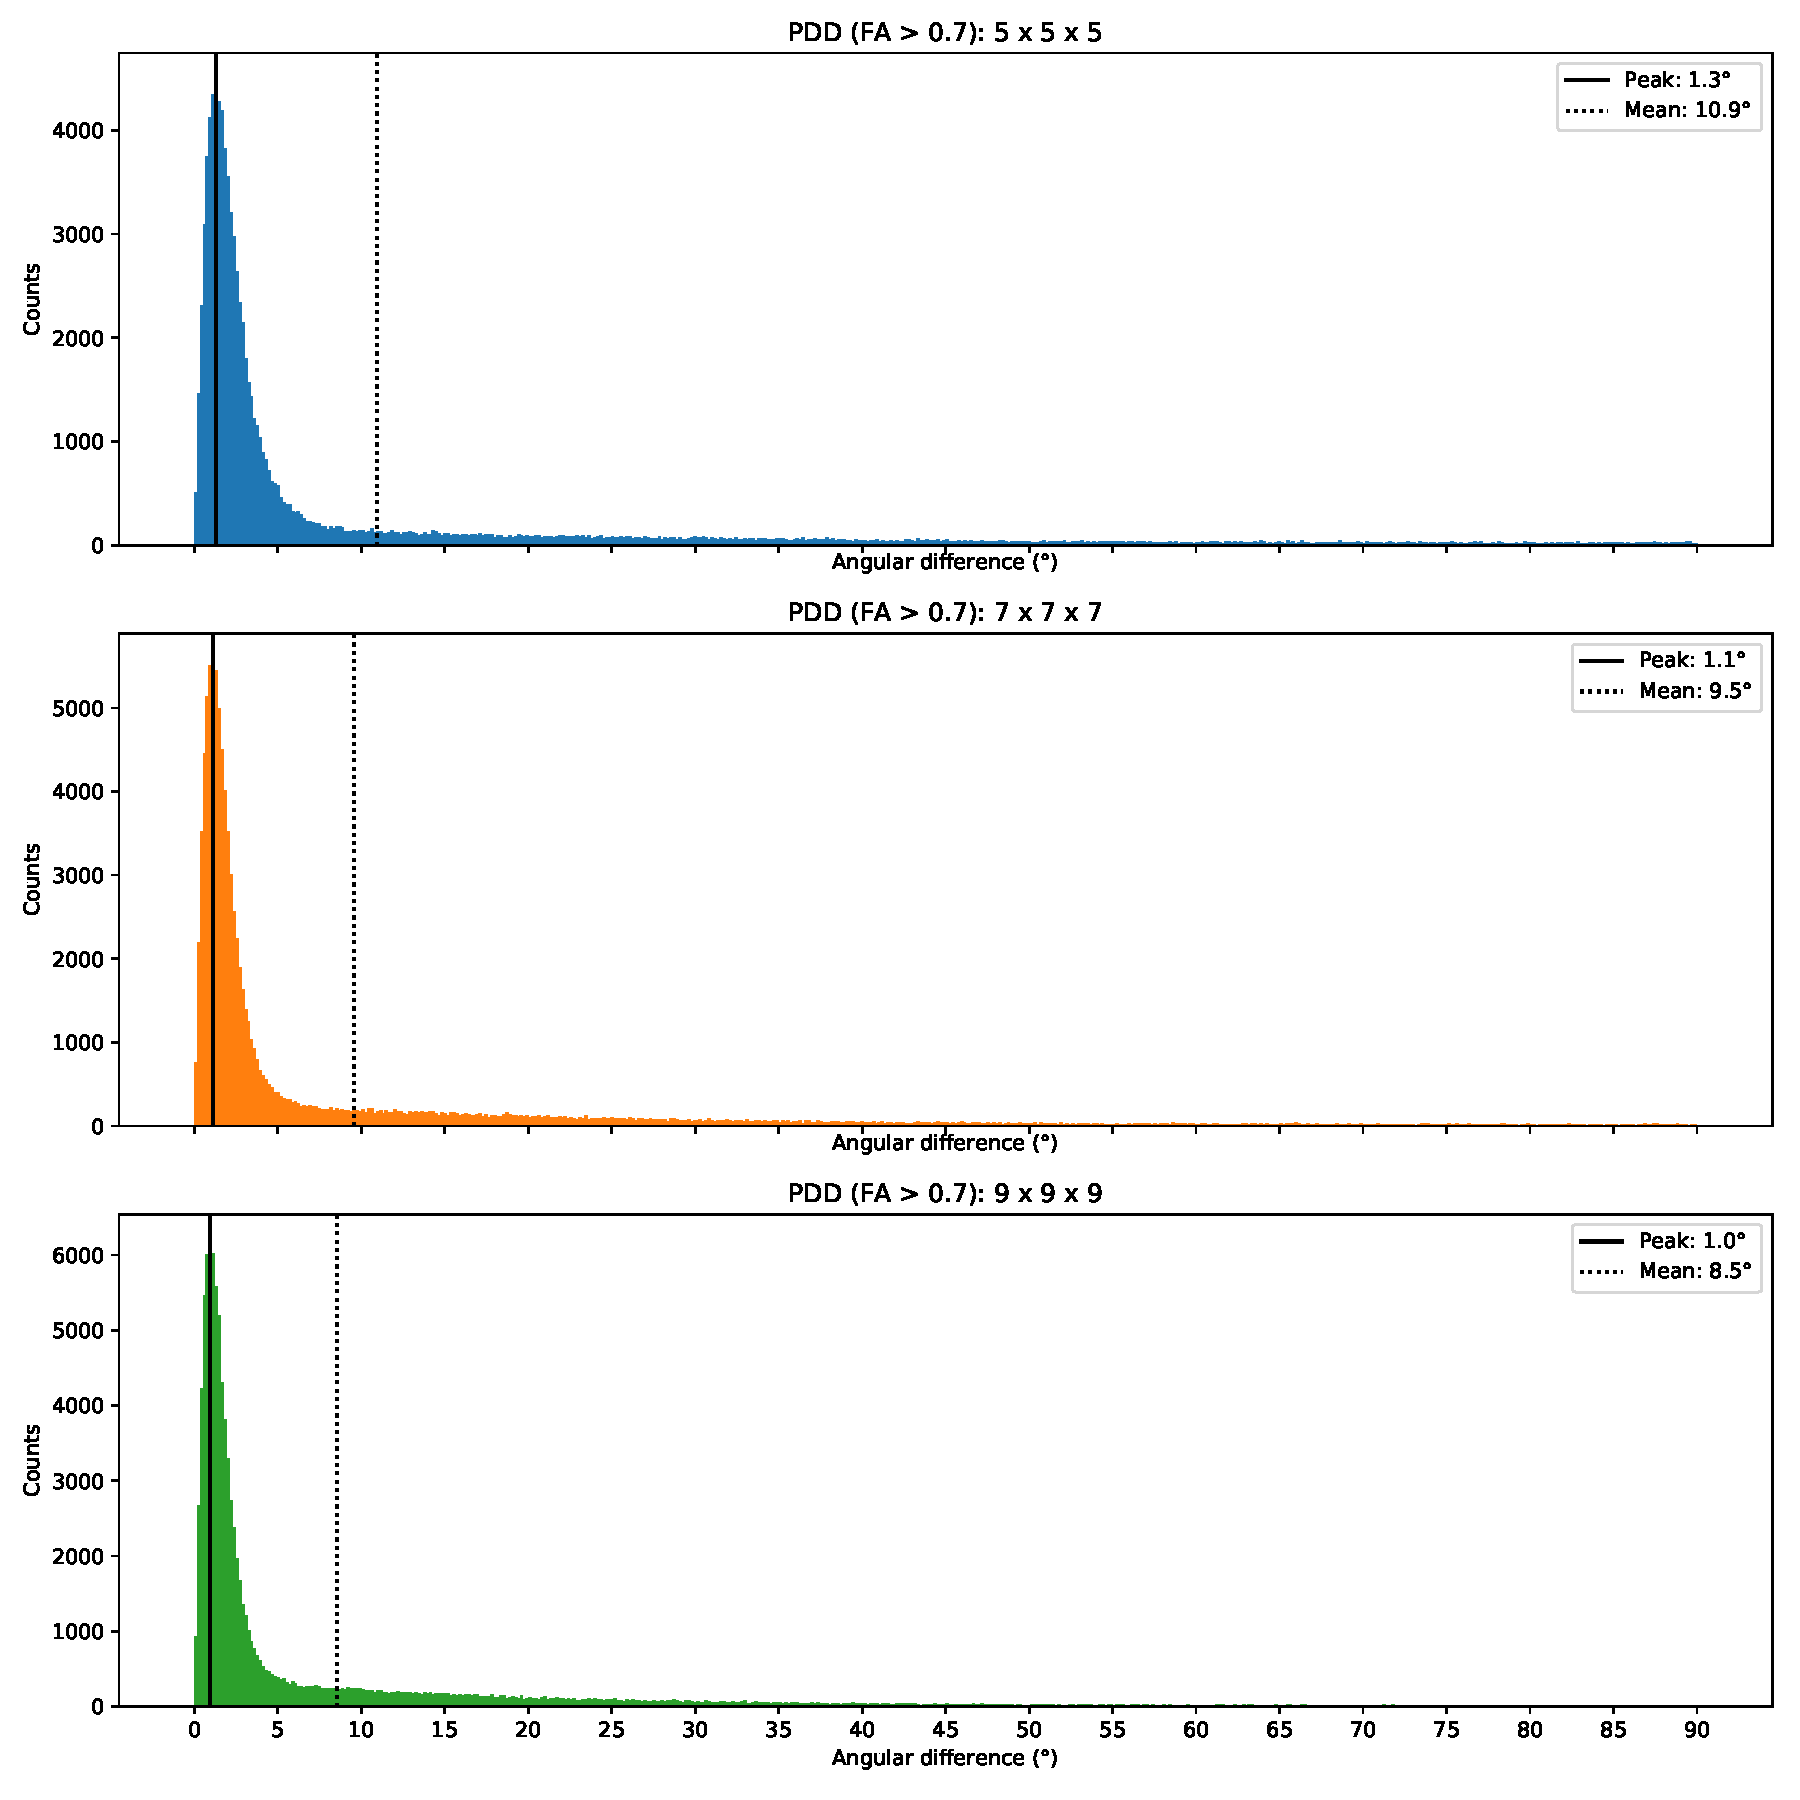
\includegraphics[width=0.6\linewidth]{../figs/noreg_pdd_famask}
  \caption{Angular difference in PDD between raw tensor fit and the denoised
    tensor fits with different window sizes. Here, comparisons were restricted
    to voxels in the brain with an FA $>$ 0.7. The bold line indicates the mean
    of the distribution, while the dotted line indicates the mean. }
  \label{fig:pdd_famask}
\end{figure}


\begin{figure}[H]
  \centering
  \captionsetup{width=0.6\linewidth}  
  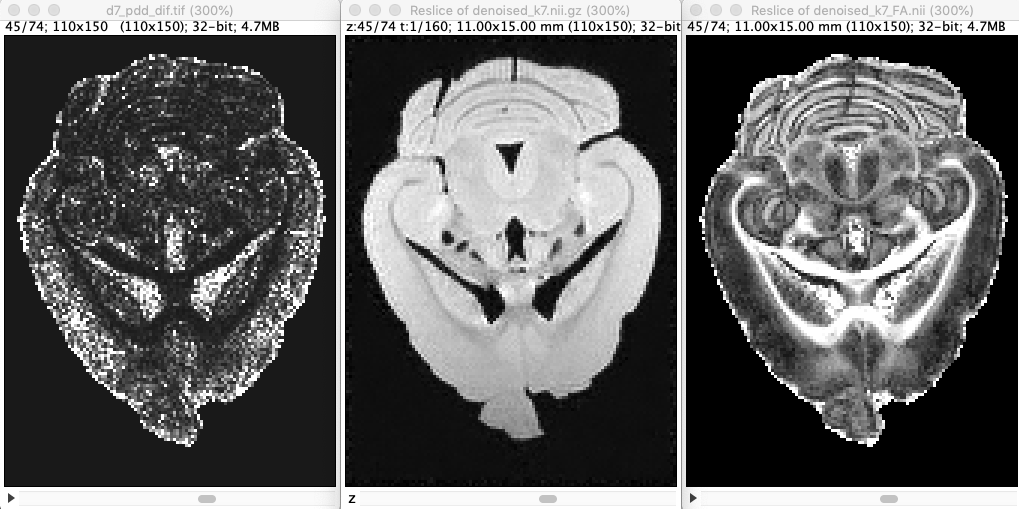
\includegraphics[width=0.6\linewidth]{../figs/pdd_diff}
  \caption{From left to right: PDD difference image, $b_0$ image, and
    FA image of the same slice. Note that areas of low PDD difference are
    in high FA regions, while areas of high PDD difference are in low
  FA areas (including the ventricles).}
  \label{fig:screenshot}
\end{figure}

\section*{Conclusion}
These results demonstrate that denoising the raw data results in a measureable
effect on the tensor fit. It is not clear how to conclude which denoising window
size is ``best'' at this point. Generally, the differences between denoised and
raw fits is much greater than the differences between fits calculated with
windows.

Next, I will look at a constrained spherical deconvolution ODF reconstruction
and see how it changes with window size. I expect to see similar
results --- that the reconstruction does not seem dramatically sensitive to the
window choice. In this case, I plan to follow the paper's
recommendation of choosing $N > M$ ($N$: voxels in the window, $M$: diffusion
directions), and use the $7\times 7 \times 7$ window to start looking into
distributions / locations of crossing fiber populations in the sample. We can
use these reconstructions to plan out where and how to section the sample before
microCT imaging if we end up needing to do that.

Once we have the microCT ground truth ODFs, we can use those as a benchmark to
evaluate all of the parameters involved in diffusion MRI processing --- denoising,
registration, the various tunable parameters in different ODF reconstruction
algorithms, etc. 

\end{document}